\chapter{Применяемые методы} \label{ch3}

Основным алгоритмом, применяемым в этой работе, является \hyperref[acr:ddpg]{градиент глубокой детерминированной политики} (Deep Deterministic Policy Gradient, DDPG), который использует архитектуру актор-критик и может работать в пространстве непрерывных действий. Поскольку сценарий игры предполагает совместную работу нескольких агентов, используется мультиагентная модификация алгоритма DDPG~---~\hyperref[acr:maddpg]{мультиагентный градиент глубокой детерминированной политики} (MADDPG). Основное его отличие, делающее его более подходящим для работы с несколькими агентами, состоит в том, что MADDPG имеет N наборов ИНС критиков-акторов, где N соответствует количеству агентов в сценарии, благодаря чему каждый агент имеет свой собственный механизм оптимизации политики. В оригинальном дизайне \cite{lowe2017multiagent} это сделано для адаптации как к совместной работе, так и к конкуренции между агентами.

Поскольку эта работа фокусируется на совместной работе нескольких агентов, тестируются несколько вариантов MADDPG, подходящих для совместной работы.

\section{Основные методы}

\subsection{Архитектура актор-критик}

Как уже упоминалось выше, алгоритм MADDPG имеет набор сетей актор-критиков для каждого агента в игровой среде. Для облегчения многоагентной совместной работы, во время тренировки, алгоритм учитывает наблюдения и действия всех агентов. Политики оптимизируются путём оценки качества, поведения всех агентов в разных состояниях среды. Таким образом, в условиях среды, требующей взаимодействия агентов, будет разработана политика, оптимальная для сотрудничества.

Глубокая нейронная сеть может рассматриваться как аппроксиматор нелинейных функций. В решении сложных задач глубокого обучения с подкреплением нейронная сеть нестабильна \cite{lillicrap2015continuous}. Эту проблему решает использование целевой (target) сети, поскольку мягкое и разрежённое обновление целевой сети замедляет её приближение к исходной сети и уменьшает влияние ошибок. Таким образом, это нарушает корреляцию между текущими и целевым Q-значениями. Хотя это снижает скорость обучения, но и улучшает стабильность обучения. В алгоритме MADDPG и у актора, и у критика есть свои целевые сети.

\subsection{Воспроизведение опыта (Experience Replay)}

Воспроизведение опыта — это механизм, когда во время тренировки в игровой среде буфер используется для сбора опыта, образцы которого из этого буфера затем случайным образом извлекаются для обучения модели.

Опыт генерируется последовательно, во время взаимодействия агентов со средой в хронологическом порядке. Неизбежно то, что собранные последовательности опыта коррелируют друг с другом. Из-за этого сеть легко переобучается на имеющиеся последовательности опыта. В итоге, переобученная сеть не может обеспечить разнообразный опыт для последующего обучения.

Опыт случайно отбирается в небольшие блоки. Это нужно не только для эффективного использования аппаратного обеспечения и увеличения скорости обучения, но также нарушает корреляцию последовательности в буфере. Таким образом, сети имеют возможность формулировать более обобщённые политики по независимым друг от друга данным.

Для применения воспроизведение опыта, в буфер, складывается опыт в виде кортежей переходов, включающих наблюдения, действия, награды и последующие наблюдения, то есть $e_t = (\mathbf{s, a, r, s'})$. Поскольку это многоагентная игровая среда, \textbf{s} - это совместные наблюдения, которые представляют собой совокупность наблюдений n агентов, $\mathbf{s} = [s_0, s_1, ..., s_n]$. То же самое относится к действиям, следующим наблюдениям и наградам. Буфер имеет ограниченную ёмкость, и при переполнении старый опыт вытесняется новым.

\subsection{Тренировка ИНС}

В то время, как агенты исследуют игровую среду, опыт перехода на каждом шаге собирается в буфер памяти. Обучение происходит только тогда, когда количество кортежей в буфере превышает определённую величину. Когда начинается обучение, \textit{актор} и \textit{критик} каждого из \textit{n} агентов обновляется на каждом шаге, в то время как \textit{целевой актор} и \textit{целевой критик} обновляются с задержкой (раз в определённое количество шагов).

На рисунке \firef{fig:ch3-network-training} показано, как обновляется набор сетей акторов-критиков. Текущее Q-значение $Q_i(\mathbf{s, a}|\theta ^Q_i)$ оценивается по сети \textit{критика}, при этом на вход подаются совместные текущие наблюдения \textbf{s} и совместные действия \textbf{a}. Целевое Q-значение $y_i$ рассчитывается из вознаграждения и дисконтированного следующего Q-значения $Q'_i(\mathbf{s', a'}|\theta ^{Q'_i})$ аппроксимированного по \textit{целевому критику}. Входные данные для сети \textit{целевого критика} – это совместные последующие наблюдения \textbf{s}' из буфера и совместные последующие действия \textbf{a}', оценённые \textit{целевыми} сетями \textit{акторов}:

\begin{equation}
    \begin{multlined}
        \mathbf{a'} = [a'_0, a'_1, ..., a'_n] \\
        = [\mu'_0(s'_0|\theta^{\mu'_0}), \mu'_1(s'_1|\theta^{\mu'_1}), ..., \mu'_n(s'_n|\theta^{\mu'_n})]
    \end{multlined}
\end{equation}

Целевое Q- значение:

\begin{equation}
    \begin{multlined}
        y_i = r_i + \gamma Q'_i(\mathbf{s', a'}|\theta^{Q'_i})
    \end{multlined}
\end{equation}

где $r_i$ это награда – \textit{i}-го агента, и $\gamma$ - это коэффициент дисконтирования или скорость затухания влияния будущих наград.

Наконец, сеть \textit{критика} обновляется путём минимизации функции потерь:

\begin{equation}
    \begin{multlined}
        L_i(\theta^{Q_i}) = \frac{1}{S} \sum (y_i - Q_i(\mathbf{s, a}|\theta^{Q_i}))^2
    \end{multlined}
\end{equation}

где \textit{S} -- это размер тренировочного набора.

\begin{figure}[ht!]
    \center
    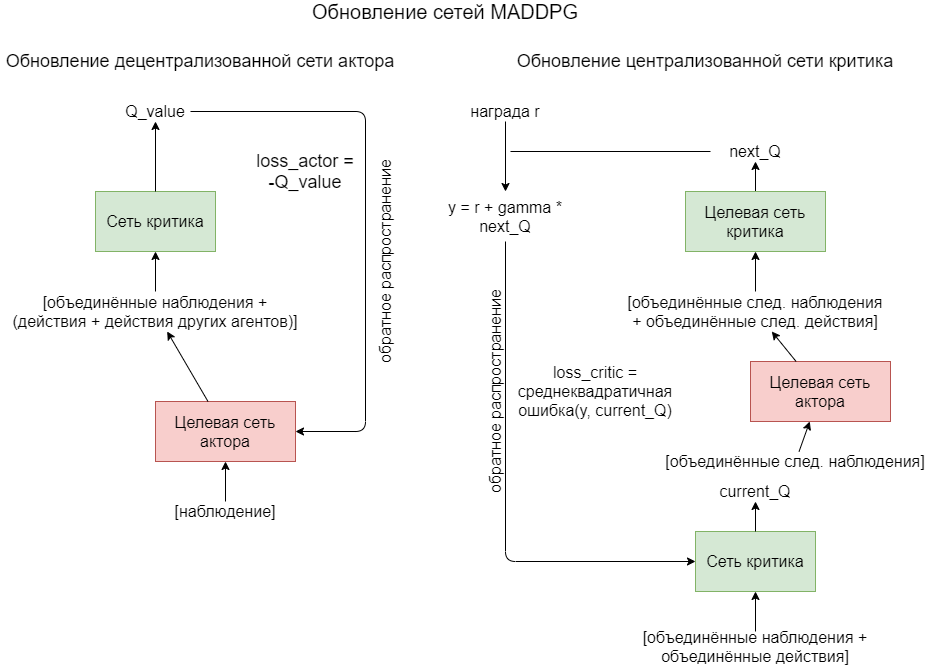
\includegraphics [scale=0.5] {my_folder/images/ch3/maddpg-updating-networks.png}
    \caption{Обновление сети \textit{актора} и \textit{критика} для каждого агента в MADDPG}
    \label{fig:ch3-network-training}
\end{figure}

Сеть \textit{актора} \textit{i}-го агента обновляется путём максимизации Q-значения сетью \textit{критика}. \textit{Критик} принимает совместные текущие наблюдения \textbf{s} из буфера и совместные текущие действия, в которых \textit{i}-е действие подменяется последним действием оценённым \textit{актором}. То есть:

\begin{equation}
    \begin{multlined}
    [a_0, a_1, a_i, ..., a_n]
        = [a_0, a_1, \mu_i(s_i|\theta^{\mu_i}), ..., a_n]
    \end{multlined}
\end{equation}

Для оптимизации уместно преобразовать задачу максимизации в задачу минимизации. Следовательно, функция потерь для обновления сети актора:

\begin{equation}
    \begin{multlined}
        L_i(\theta^{\mu_i}) = -Q_i(\mathbf{s}, [a_0, a_1, \mu_i(s_i|\theta^{\mu_i}), ..., a_n]|\theta^{Q_i})
    \end{multlined}
\end{equation}

Сети \textit{целевых актора} и \textit{критика} обновляются не полным копированием сетей \textit{актора} и \textit{критика}, а с использованием \textit{мягкого обновления} (soft update):

\begin{equation}
    \begin{multlined}
        \theta^{\mu'_i} = \tau \theta^{\mu_i} + (1 - \tau)\theta^{\mu'_i}\\
        \theta^{Q'_i} = \tau \theta^{Q_i} + (1 - \tau)\theta^{Q'_i}
    \end{multlined}
\end{equation}

где $\tau$ обычно очень мала, например 0.01 в этой работе.

\section{Прикладные методы}

\subsection{Архитектура ветвления действий (Action Branching)}

В сценариях, подразумевающих совместную работу нескольких агентов наряду с физическими действиями важно иметь и коммуникационные действия. В некоторых случаях количество действий может быть большим, как в \cite{tavakoli2017action}. В игровых сценариях этой работы агент имеет два вида действия, которые представляют физическое движение и действие, выбранное для общения.

Полное действие в таких сценариях включает в себя два относительно независимых действия. Сеть \textit{акторов} проектируется таким образом, что она выделяет скрытые представления из наблюдений и имеет две «головы» на выходе. Одна возвращает физическое действие, вторая – действие для общения.

В соответствии с теорией архитектуры ветвления действий \cite{tavakoli2017action}, можно оптимизировать каждое измерение действия относительно независимо. Полное действие в итоге представляет собой объединение двух действий.

\subsection{Исследовательский шум (Exploration Noise)}

\textit{Исследование} и \textit{эксплуатация} (Exploration and exploitation) — это дилемма в обучении с подкреплением. \textit{Эксплуатация} — это когда агент следует текущей политике, чтобы совершать жадные действия, которые приносят наибольшую награду. \textit{Исследование} берет на себя риски, чтобы попробовать другие действия, которые потенциально могут принести лучшую награду в долгосрочной перспективе. \textit{Исследование} необходимо агенту, ищущему оптимальную политику, хотя оно кажется неоптимальным в нынешней ситуации и дает меньшее вознаграждение. В обучении с подкреплением агент обычно больше \textit{исследует} окружающую среду в начале обучения. В ходе оптимизации политики с течением времени, агент постепенно уменьшает и стабилизирует \textit{исследование} до низкого уровня, и в итоге больше придерживается получившейся оптимальной политики.

Чтобы включить \textit{исследование}, на действия накладываются шумы. Какой шум применять, определяется настройкой среды. \textit{Процесс Орнштейна-Уленбека} используется в DDPG в [2] для получения коррелированных по времени \textit{исследований}. Он считаются, эффективным для проблем физического контроля с инерцией. Гауссовское распределение шума используется для физических движений в [4]. В этой работе для наложения шума на действия, генерируемые сетью \textit{акторов} выбирается стандартное \textit{Гауссовское распределение}.

\begin{equation}
    \begin{multlined}
        \mu'_i(s_i) = \mu_i(s_i|\theta^{\mu_i}) + \mathcal{N}
    \end{multlined}
\end{equation}

где $\mu'$ - политика исследования, а $\mathcal{N}$ - шум исследования, который можно выбрать в зависимости от настроек среды. $\mathcal{N}$ затухает на каждом шаге со скоростью $\epsilon$, то есть $\mathcal{N} \leftarrow \epsilon \mathcal{N}$.

\section{Варианты алгоритмов}

\subsection{MADDPG с декомпозированным вознаграждением (Decomposed Reward)}

Предполагается сценарий игры, в котором агенты выполняют относительно независимые под-действия, каждое под-действие может воздействовать на среду и приводить к вознаграждению, которое отделено от глобального вознаграждения. Идея декомпозирования награды MADDPG в том, что для каждого под-действия может быть сформулирована независимая политика. Каждый агент, имеет \textit{n} независимых наборов сетей \textit{актор-критиков}, каждый из которых соответствует одному виду действия. Ожидается, что политики для отдельных видов действий могут быть оптимизированы путем обучения соответствующих групп критиков.

В этой работе планируется использовать этот вариант в сценарии \textit{Simple Reference}.

\subsection{MADDPG с общим мозгом}

Другой вариант MADDPG вдохновлен \cite{mordatch2017emergence}. В этом варианте есть только один набор сетей \textit{акторов-критиков}, который используется всеми агентами. Это подразумевает, что все агенты имеют одинаковую оптимальную политику. Этот подход использует предположение о том, что все агенты имеют одно и то же пространство действий и пространство наблюдений, и они также имеют общую глобальную награду. Этот подход особенно эффективен для коммуникационных действий, поскольку композиционный язык постоянно появляется среди всех участников игрового сценария. В варианте с общим набором сетей все агенты говорят на одном языке, в отличие от стандартного MADDPG, где каждый агент может интерпретировать один и тот же ориентир по-разному. Это особенно важно, когда сотрудничают более двух агентов, поскольку им нужно общаться на одном языке.


\section{Выводы}

В этой главе были рассмотрены методы, которые были выбраны для исследования. Именно эти методы, подходы и алгоритмы были задействованы в экспериментах, речь о которых пойдёт в следующей главе. 

Сценарии, в которых производились эксперименты, уже упоминались в \hyperref[intro:sec2]{1.2 Сценарии}. Более подробно они так же будут рассмотрены в следующей главе.

\newpage
